\documentclass[12pt]{article}
%%%%%%begin preamble
\usepackage[hmargin=1in, vmargin=1in]{geometry} % Margins
\usepackage{hyperref}
\usepackage{url}
\usepackage[numbers]{natbib}
\usepackage{graphicx}
\usepackage{amsmath}
\usepackage{amsfonts}
\usepackage{amssymb}
\usepackage{wrapfig}

\usepackage{multicol}
\usepackage{etoolbox}
%\patchcmd{\thebibliography}{\section*{\refname}}
%    {\begin{multicols}{2}[\section*{\refname}]}{}{}
%\patchcmd{\endthebibliography}{\endlist}{\endlist\end{multicols}}{}{}


\usepackage[normalem]{ulem}
\usepackage{xcolor}
\newcommand{\edit}[2]{\textcolor{purple}{\sout{#1} \textbf{#2}}}

\hypersetup{
  colorlinks   = true,
  %citecolor    = blue
  citecolor    = blue
  % gray is not being found!?!
  % gray is found if pdfpages is used... crap.
  %citecolor    = grey
  %citecolor    = Gray
}


%% headers
\usepackage{fancyhdr}
\pagestyle{fancy}
\fancyhf{} % sets both header and footer to nothing
\lhead{Evan H. Anders}
\rhead{Research Statement}
\cfoot{\footnotesize{\thepage}}
%\pagestyle{empty}
%\pagenumbering{gobble}
%\renewcommand*{\thefootnote}{\fnsymbol{footnote}}

\renewcommand{\vec}{\ensuremath{\boldsymbol}}
\newcommand{\dedalus}{\href{http://dedalus-project.org}{Dedalus}}
\newcommand{\del}{\ensuremath{\vec{\nabla}}}
\newcommand{\scrS}{\ensuremath{\mathcal{S}}}

\newcommand{\prf}{PRF}
\newcommand{\prr}{PRR}
\newcommand{\ssr}{SSR}
\newcommand{\araa}{ARAA}
\newcommand{\mnras}{MNRAS}
\newcommand{\aap}{A\&A}
\newcommand{\apjl}{ApJL}
\newcommand{\apj}{ApJ}
\newcommand{\apjs}{ApJL}

\newcommand{\sct}[1]{\vspace{0.3cm}\hspace{-\parindent}\textbf{\underline{#1}}\hspace{0.3cm}}

%\newcommand{\nosection}[1]{%
%  \refstepcounter{section}%
%  \addcontentsline{toc}{section}{\protect\numberline{\thesection}#1}%
%  \markright{#1}}
%\newcommand{\nosubsection}[1]{%
%  \refstepcounter{subsection}%
%  \addcontentsline{toc}{subsection}{\protect\numberline{\thesubsection}#1}%
%  \markright{#1}}

%\usepackage{atbegshi}
%%%%%%end preamble


%Make bibliography 2col
\bibliographystyle{apj_small}
\makeatletter
\renewenvironment{thebibliography}[1]
     {\begin{multicols}{2}[\paragraph*{\refname}\vspace{-0.1in}]%
      \@mkboth{\MakeUppercase\refname}{\MakeUppercase\refname}%
      \list{\@biblabel{\@arabic\c@enumiv}}%
           {\settowidth\labelwidth{\@biblabel{#1}}%
            \leftmargin\labelwidth
            \advance\leftmargin\labelsep
            \@openbib@code
            \usecounter{enumiv}%
            \let\p@enumiv\@empty
            \renewcommand\theenumiv{\@arabic\c@enumiv}}%
      \setlength{\itemsep}{-2pt}
      \sloppy
      \clubpenalty4000
      \@clubpenalty \clubpenalty
      \widowpenalty4000%
      \sfcode`\.\@m}
     {\def\@noitemerr
       {\@latex@warning{Empty `thebibliography' environment}}%
      \endlist\end{multicols}}
\makeatother



\begin{document}
\thispagestyle{fancy}

\sct{Context \& Aims}
Current and next-generation space- and ground-based observatories are revolutionizing precision observations in astrophysics.
Discoveries ranging from exoplanets to black holes rely on high-precision stellar evolution models for calibration \citep{mesa6}, and convection introduces uncertainty into these models.
Mixing at the convective core boundary of massive stars ($M_* \gtrsim 1.1 M_\odot$) leads to core mass uncertainties of up to 70\% \citep{kaiser_etal_2020}, making the evolutionary pathway of a star from birth to death unclear.
Convective motions near this boundary generate gravity waves which propagate towards the stellar surface and provide one of the few tools for probing the structure of stars via asteroseismology.
The nonlinear 3D convection that drives these processes is poorly modeled in stellar evolution calculations.

\textbf{The goal of my research plan is to build a next-generation set of global and local 3D numerical simulations, which will answer the following questions:}\vspace{-0.2cm}
\begin{enumerate}
    \item How large are convective cores in massive stars? \vspace{-0.2cm}
    \item How does rotation and boundary mixing affect the generation and observable spectrum of gravity waves in massive stars?
\end{enumerate}

\sct{My Prior Research}
My research is rooted in fluid dynamics and inspired by observations of stars.
I use the \emph{Dedalus} \citep{burns_etal_2020} pseudospectral code to design and run state-of-the-art simulations which I use to learn about mixing processes like convection in stars.
\textbf{A core focus of my research has been to push the boundaries of \emph{time} evolution, while other studies have focused on \emph{spatial} resolution; my focus on the time domain has led to key discoveries in my career.}
When I was a graduate student, I focused on fundamental studies of convection.
I studied heat transport in compressible convection with  \citep{anders_etal_2019_rot} and without \citep{anders_brown_2017} rotation.
I studied how fast convection interacts with the slow evolution of the background thermal structure in convective regions \citep{anders_etal_2018,anders_etal_2020}.
I also studied convection at the smallest scales, examining individual downflows in the Sun's convection zone \cite{anders_etal_2019_thermals}.
As a postdoctoral fellow at Northwestern, I have connected my theoretical research with modern observational puzzles.
I have formed collaborations with observers and 1D modelers alike to understand what sets the position of a convective boundary \citep{anders_etal_2022b}, and I have discovered the process that inflates the convective cores of stars relative to standard models \citep{anders_etal_2022a}.
I am now finishing a project focusing on gravity wave generation by core convection and the observable signals of these waves, for direct comparison with e.g., asteroseismic observations.


\sct{Future Focus I: Convective Boundary Mixing}
Observations demonstrate a need for improved models of convective boundary mixing (CBM) \citep{johnston2021}.
For example, an unexplained mass-dependent CBM is required to reproduce observed eclipsing binary populations  \citep{claret_torres_2019}.
Asteroseismology allows us to directly probe near-core CBM, revealing extensive mixing occurs near convective core boundaries \citep{michielsen_etal_2019, pedersen_etal_2021}.
The amount of CBM used in a stellar evolution model modifies the evolution of a star's luminosity and effective temperature as well as the mass of the eventual remnant that it leaves behind \citep{castro_etal_2014,higgins_vink_2019}.


To understand the fluid dynamical picture behind CBM, I will create simulations of the cores of massive stars using the \emph{Dedalus} \citep{burns_etal_2020} code.
These simulations will differ from past simulations of massive stars, because they will include the full ``ball'' geometry of the convective core, they will employ the fully compressible equations without any luminosity boosting, and they will be relaxed into thermal equilibrium (See Fig.~\ref{fig:star} for a preliminary example of one of these simulations).
\emph{Dedalus} was recently updated with the state-of-the-art ability to simulate flows that pass through the coordinate singularity at $r = 0$ in spherical coordinates \citep{vasil_etal_2019,lecoanet_etal_2019}; most prior codes used a spherical shell geometry with a small interior ``cutout'' of the core.
Our implicit-explicit (IMEX) timestepping scheme allows us to circumvent timestepping restrictions from fast sound waves \citep{anders_brown_2017}, so we can take fast timesteps without boosting the luminosity as many prior simulations have done.
Evolving a simulation to thermal equilibration using classic timestepping techniques can take thousands of convective overturn timescales \citep{anders_etal_2022a,anders_etal_2022b}.
Fortunately, I have developed methods of ``accelerated evolution'' \citep{anders_etal_2018}, which self-consistently equilibrate simulations using an order of magnitude fewer cpu-hours than traditional timestepping.



\begin{wrapfigure}{r}{0.5\textwidth}
  \begin{center}
      \vspace{-1.6cm}
    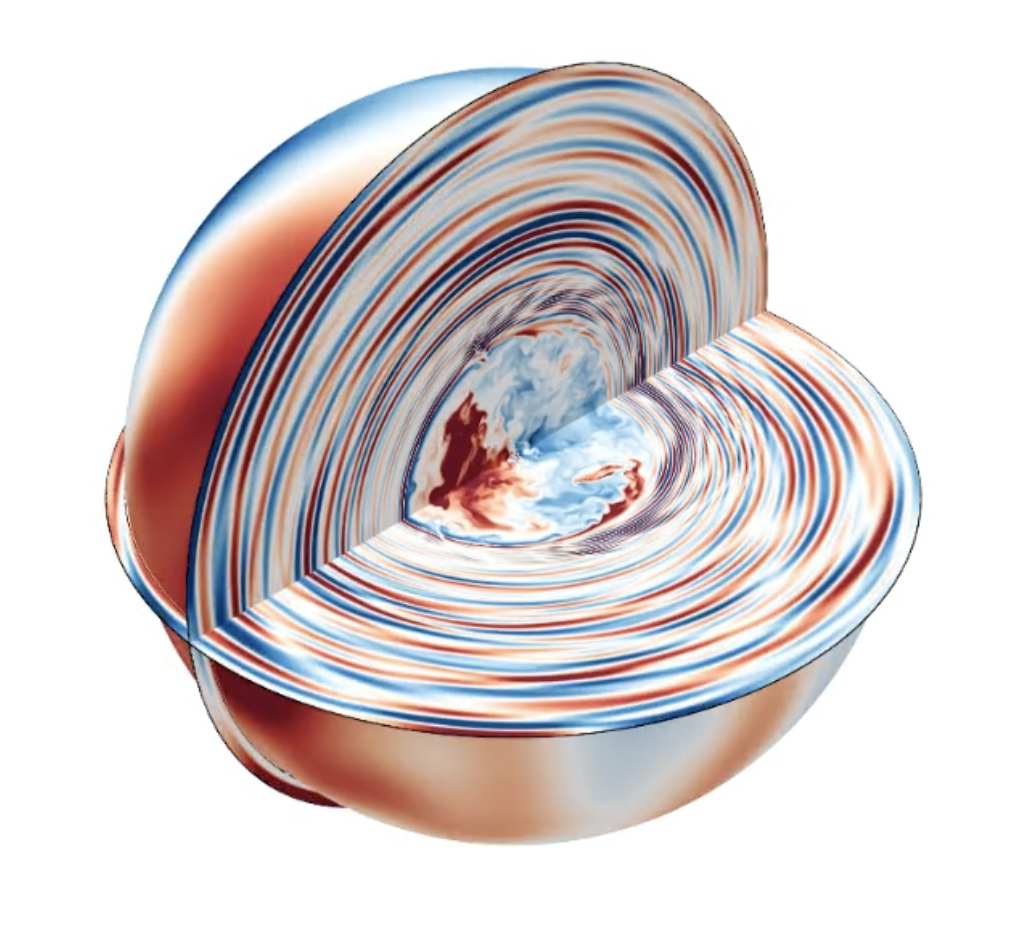
\includegraphics[width=0.45\textwidth]{dedalus_massive_star.png}
      \vspace{-1.3cm}
  \end{center}
    \caption{A simulation I ran in \emph{Dedalus} of a {$40 \,M_{\odot}$} star. 
    The entropy field is visualized; red is hot and buoyantly rises, blue is cold and falls. 
    We see a convective core with a strong dipole flow and an outer radiative envelope with internal gravity waves. \label{fig:star}}
    \vspace{-0.5cm}
\end{wrapfigure}
I will study CBM in fully compressible simulations whose background stratifications are based upon \emph{MESA} (Modules for Experiments in Stellar Astrophysics) models of massive stars.
I will study non-rotating and rotating stars with masses varying in the range $M_* = 1.1-40 M_{\odot}$ (the lowest masses where convective cores appear, up to high masses).
My results will calibrate a 1D implementation of convective boundary mixing, which I will then implement into the open-source \emph{MESA} software instrument.
Throughout this process, I will build my simulation code with ease-of-use for the user in mind, and this code will be made publicly available and citeable so that the community has access to a robust tool for studying fluid dynamics in massive stars.

\textbf{\underline{\emph{Deliverable:}} The first rotating, 3D simulations of core convection that include $\boldsymbol{r = 0}$ and reach thermal equilibrium.}

\sct{Future Focus II: Core-generated Gravity Waves}
Gravity wave pulsations of intermediate mass stars have recently been used to probe the radial distribution of mixing in those stars \citep{pedersen_etal_2021}.
Direct comparisons between observed wave peaks in photometric spectra \citep{decat_aerts_2002, pedersen_etal_2021} and those produced by 3D simulations of stars have not been performed.
Most simulations of gravity waves in massive stars in recent years \citep{edelmann_etal_2019,horst_etal_2020} have focused on trying to explain ``red noise'' \citep{bowman_etal_2019} observed at the surfaces of hot, massive stars rather than the peaks in the spectra of $\gamma$ Dor and SPB stars.
I am currently working to understanding the spectrum of waves generated by core convection and the expected surface appearance of these waves in non-rotating stars like the one pictured in Fig.~\ref{fig:star}.

All massive stars rotate rapidly \citep{jermyn_etal_2022_atlas}, and this rotation affects both the convective dynamics \citep{aurnou_etal_2020} and the observable waves \citep[e.g.,][]{papics_etal_2017}.
I will add rotation to simulations like those in Fig.~\ref{fig:star} to create the first-ever simulations of rotating, 3D core convection to understand both how rotation modifies the convective flows (and thus the spectrum of waves they generate), as well as the observable signal of these waves at the surface.
In light of increasing evidence for nearly-adiabatic, well-mixed ``convective penetration'' CBM zones at the boundaries of massive stars' cores \citep{pedersen_etal_2021,anders_etal_2022a}, I will also study how the presence of a convective penetration zone changes the excitation of gravity waves.
These waves are generally driven by a cascade of turbulent eddies acting on an evanescent tail of the wave at the boundary of the convection zone.
These convective penetration zones are odd in that wave modes can stably extend into them before becoming evanescent in the bulk convective region.
This may significantly alter the manner in which waves are driven, particularly at the largest, most observable scales.
Throughout this study, I will synthesize observables of the wave spectrum at the stellar surface and compare my results to asteroseismic measurements of $\gamma$ Dor and SPB stars.

\textbf{\underline{\emph{Deliverable:}} The first 3D, spherical simulations of core gravity wave generation including rotation or extended mixing regions.}

\sct{The CCA as the ideal location for the next stage of my career}
I would love to join the CCA for many reasons.
I want to work somewhere that values creating open source, accessible, high-impact research software.
I want to create widely-used modules both for plotting and post-processing \emph{Dedalus} results and for creating and running 3D global simulations of stars like the one in Fig.~\ref{fig:star}.
Being an FRF at the CCA would provide me with the structure and support required to create these modules.

My research most naturally fits into the Stars \& Compact Objects group, and I would collaborate with Dr.~Cantiello on the research proposed here.
I focus my work on the progenitors of compact objects which can now be observed through gravitational wave interferometers, and I hope also to plug in to the Gravitational Wave Astronomy group to learn more about constraints that gravitational wave astronomy places on my work.
I also envision productive collaboration with the Planet Formation group (discussion of research questions and simulation techniques with e.g., Drs.~Armitage and Jiang) and the Astronomical Data group (I am keen to learn about challenges for stellar models in describing large populations).

I have used the extremely flexible \emph{Dedalus} code for eight years; outside of the five core developers, I am the leading Github contributor to the code base.
I know \emph{Dedalus} inside and out, and would be happy to provide support to any other members of the Simons Foundation who are interested in using a flexible and general PDE solver like \emph{Dedalus} on their own research problems.
\emph{Dedalus} has been used to study dynamics in quantum superfluids and the formation of bacterial sheets, and I would be excited about opportunities to use my knowledge of \emph{Dedalus} to form collaborations with the CCB or CCQ.

\vspace{-0.3cm}
{\scriptsize
\bibliography{biblio}
}
\end{document}
